
\documentclass[12pt,a4paper]{article} 

\usepackage{float,times,graphicx,mathtools}
\usepackage{amsmath}
\usepackage{amsfonts}
\usepackage{amssymb}
\usepackage{latexsym}
\usepackage{epsfig}
\usepackage{graphicx}
\usepackage{caption}
\usepackage{subcaption}
\usepackage{color}
\usepackage{pdfpages}
\usepackage{natbib}
\usepackage[space]{grffile}
\usepackage{wrapfig}
\usepackage{subcaption}
\usepackage{url}
\usepackage{bbm}
\usepackage{tikzsymbols}

\DeclareMathOperator{\logit}{logit}
\DeclareMathOperator{\tr}{tr}
\bibpunct[, ]{(}{)}{;}{a}{,}{,}
\graphicspath{{../}}  
\addtolength{\oddsidemargin}{-1in}
	\addtolength{\evensidemargin}{-1in}
	\addtolength{\textwidth}{1.75in}
	\addtolength{\topmargin}{-1.3in}
	\addtolength{\textheight}{2in}
\date{\vspace{-5ex}}
\begin{document}


\begin{itemize}
\item Tried different priors on the LogQuad $h$ parameter, AR(1) around IGME estimates, MVN around IGME estimates, weighted means on IGME estimates, AR(1) around common mean, ARIMA(1,1,0) 
	\begin{itemize}
	\item[--] used WPP population estimates at 1960, 1975, 1985, 1995, 2005 and 2015 as input
	\item[--] IGME estimates seem to be inconsistent with the population data/DHS data
	\item[--] at years where there is no population data, the IGME based priors do have an effect and draw the fitted $\boldsymbol{h}_t$ towards the IGME estimates, but at years with population data the estimates just drop and move further away from the IGME estimates
	\item[--] tried fitting the same model with MVN prior around the IGME estimates without using the DHS data, and the estimated $\boldsymbol{h}_t$ deviates even further away from the IGME estimates, so the inconsistency probably mainly comes from the population counts instead of the DHS data 
	\item[--] prior contribution of different dimensions? $\boldsymbol{h}_t$ and $\boldsymbol{g}_{xt}$
	\end{itemize}
	
\item used UNPD census counts at 1975, 1985, 1996 and 2006 instead (keeping WPP 1960 estimates as baseline) and TMB cannot converge (outer mgc is NaN/NA) in some cases, e.g. MVN around IGME estimates and weighted means on IGME estimates
\begin{itemize}
\item[--] assumed constant intercensal grow rates in population counts to extrapolate
\item[--] cannot figure out which parameter(s) are causing problems yet
\item[--] the MVN prior converges when I do not use IGME estimates as prior means, and estimate a common mean instead
\end{itemize}
\end{itemize}

\begin{figure}[H]
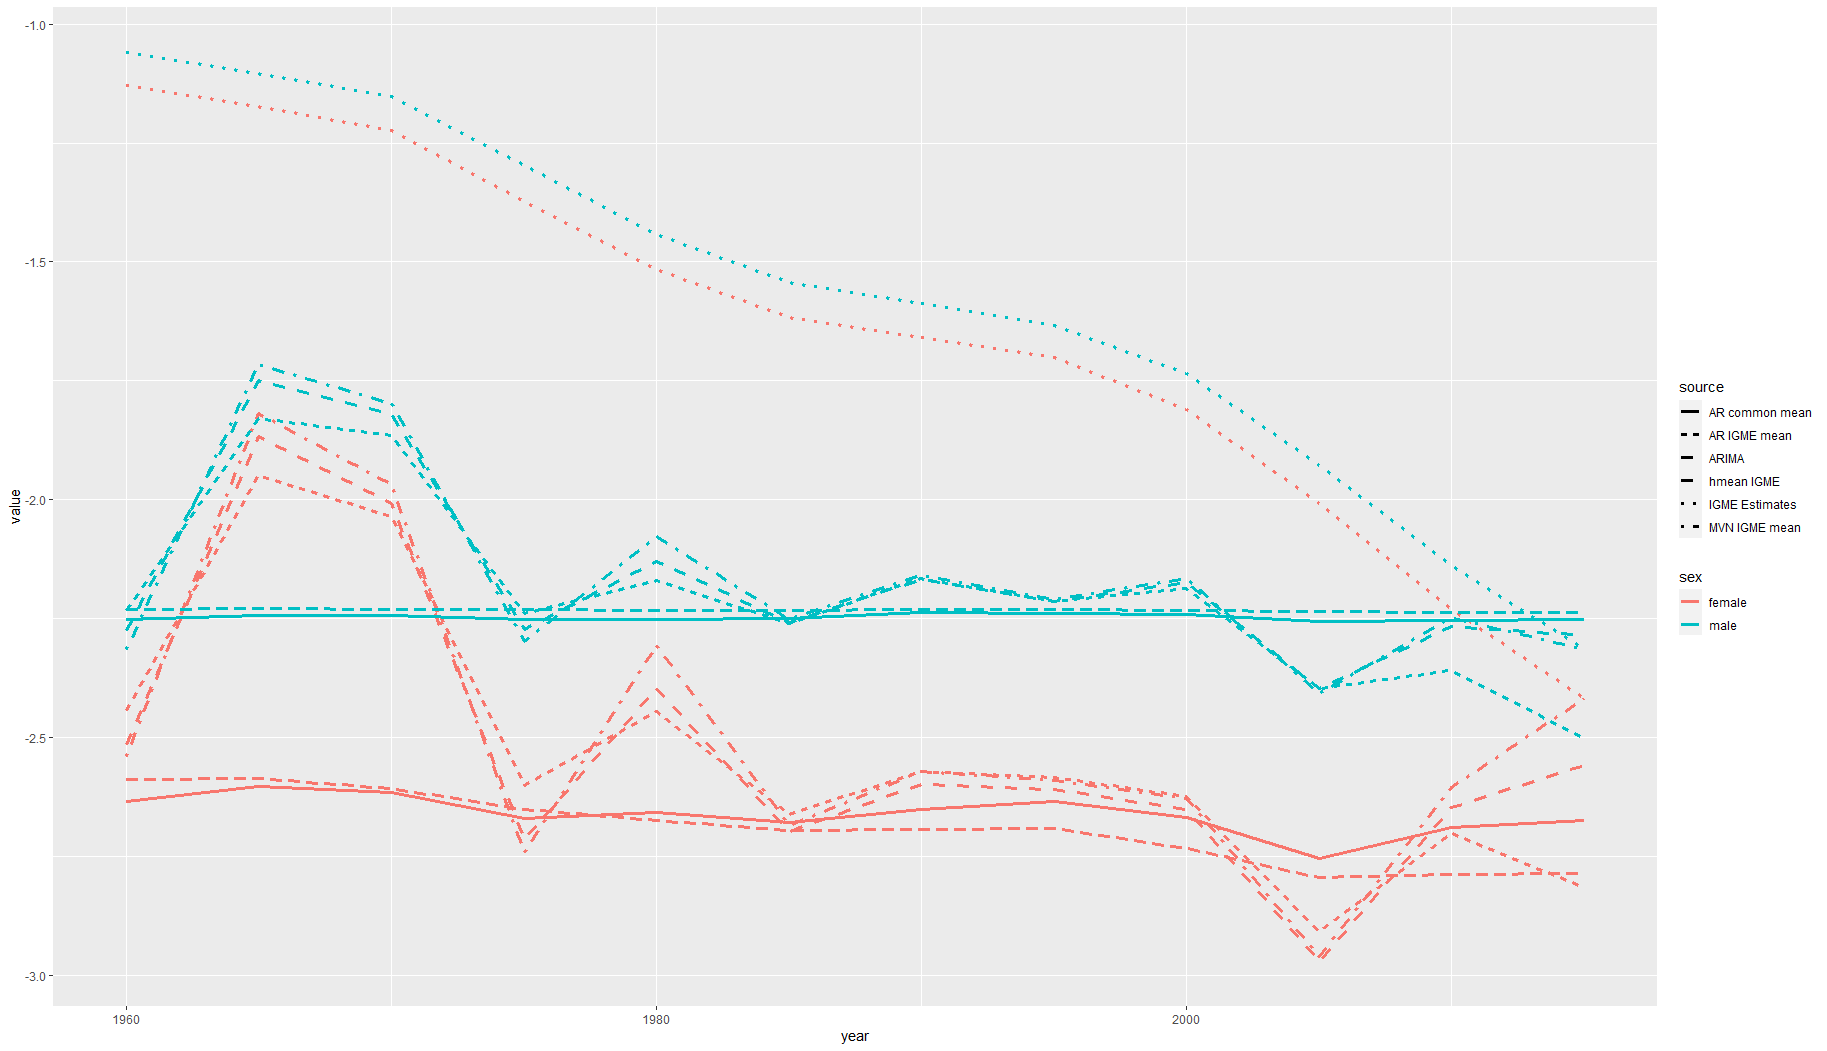
\includegraphics[width = \linewidth]{Burkina Faso/h priors.jpg}
\end{figure}
\end{document} 